\section*{Pourquoi apprendre NoSQL ? }

\subsection*{Les limites du relationnel dans le monde moderne}

\begin{frame}{Pourquoi apprendre NoSQL ? À quoi ça sert ?}
    \begin{figure}[htb]
        \centering
        \begin{tikzpicture}

            \node[inner sep=0pt, label=below:Volume] (volume) at (0,0)
                {
\includegraphics[width=.2\textwidth]{img/icon/volume.png}};

            \node[inner sep=0pt, label=below:Données non-structurées, right=of volume, xshift=2cm] (unstructured)
                {
\includegraphics[width=.2\textwidth]{img/icon/unstructured.png}};

            \node[inner sep=0pt, label=below:Scalabilité, below=of volume, yshift=-1cm] (scale)
                {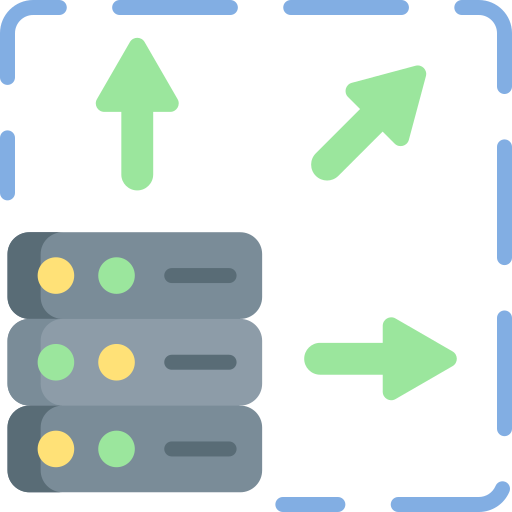
\includegraphics[width=.2\textwidth]{img/icon/scale.png}};

            \node[inner sep=0pt, label=below:Latence, right=of scale, xshift=2cm] (latency)
                {
\includegraphics[width=.2\textwidth]{img/icon/latency.png}};
        \end{tikzpicture}
    \end{figure}

    \note{
        Les bases de données relationnelles excellent pour des données structurées, stables et peu volumineuses. Mais elles montrent leurs limites dans des contextes où :

        \begin{itemize}
            \item Le volume de données explose : les tables relationnelles deviennent lentes et coûteuses à faire évoluer.
            \item Les données sont non structurées ou variées : JSON, logs, vidéos, messages, etc. ne rentrent pas dans un schéma fixe.
            \item La scalabilité horizontale est nécessaire : ajouter des serveurs pour gérer la charge est complexe avec les BDR.
            \item La latence doit être ultra-faible : les requêtes complexes (jointures) ralentissent les applications temps réel.
        \end{itemize}
    }

\end{frame}

\begin{frame}{Statistiques récentes sur l’adoption de NoSQL}

    \begin{figure}[htb]
        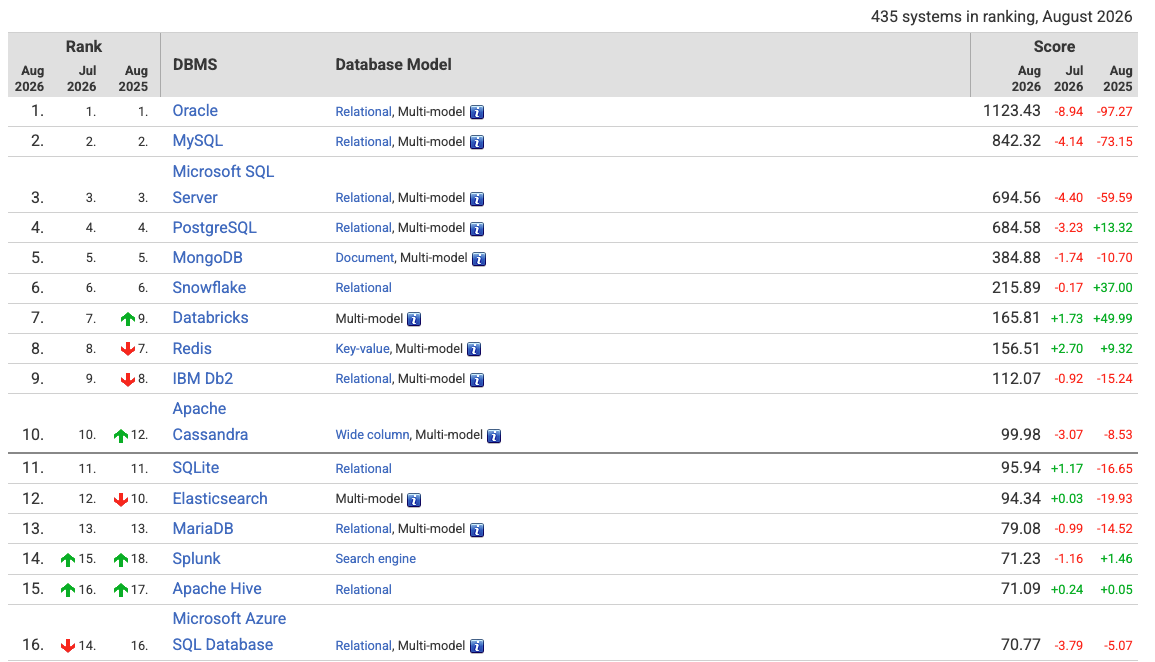
\includegraphics[width=\textwidth]{img/db-engine-ranking.png}
        \caption{Popularité des bases de données en août 2026\\\vspace{0.1cm}Source : DB Engines Ranking}
    \end{figure}

    \note{
            \begin{itemize}
            \item DB-Engines Ranking (2026) :  MongoDB, Redis et Cassandra figurent parmi les 10 bases de données les plus populaires au monde, avec une croissance annuelle de 20 à 30\% depuis 2020.
                \begin{itemize}
                    \item MongoDB : 5e position (source : \href{https://db-engines.com/en/ranking}{DB-Engines, août 2026})
                    \item Redis : 7e position
                    \item Cassandra : 10e position
                \end{itemize}
            \item Marché : le marché des bases NoSQL devrait atteindre 22 milliards de dollars d’ici 2027 (source : MarketsandMarkets).
            \end{itemize}
    }
\end{frame}

\begin{frame}{Adoption de NoSQL}
    \begin{figure}[htb]
        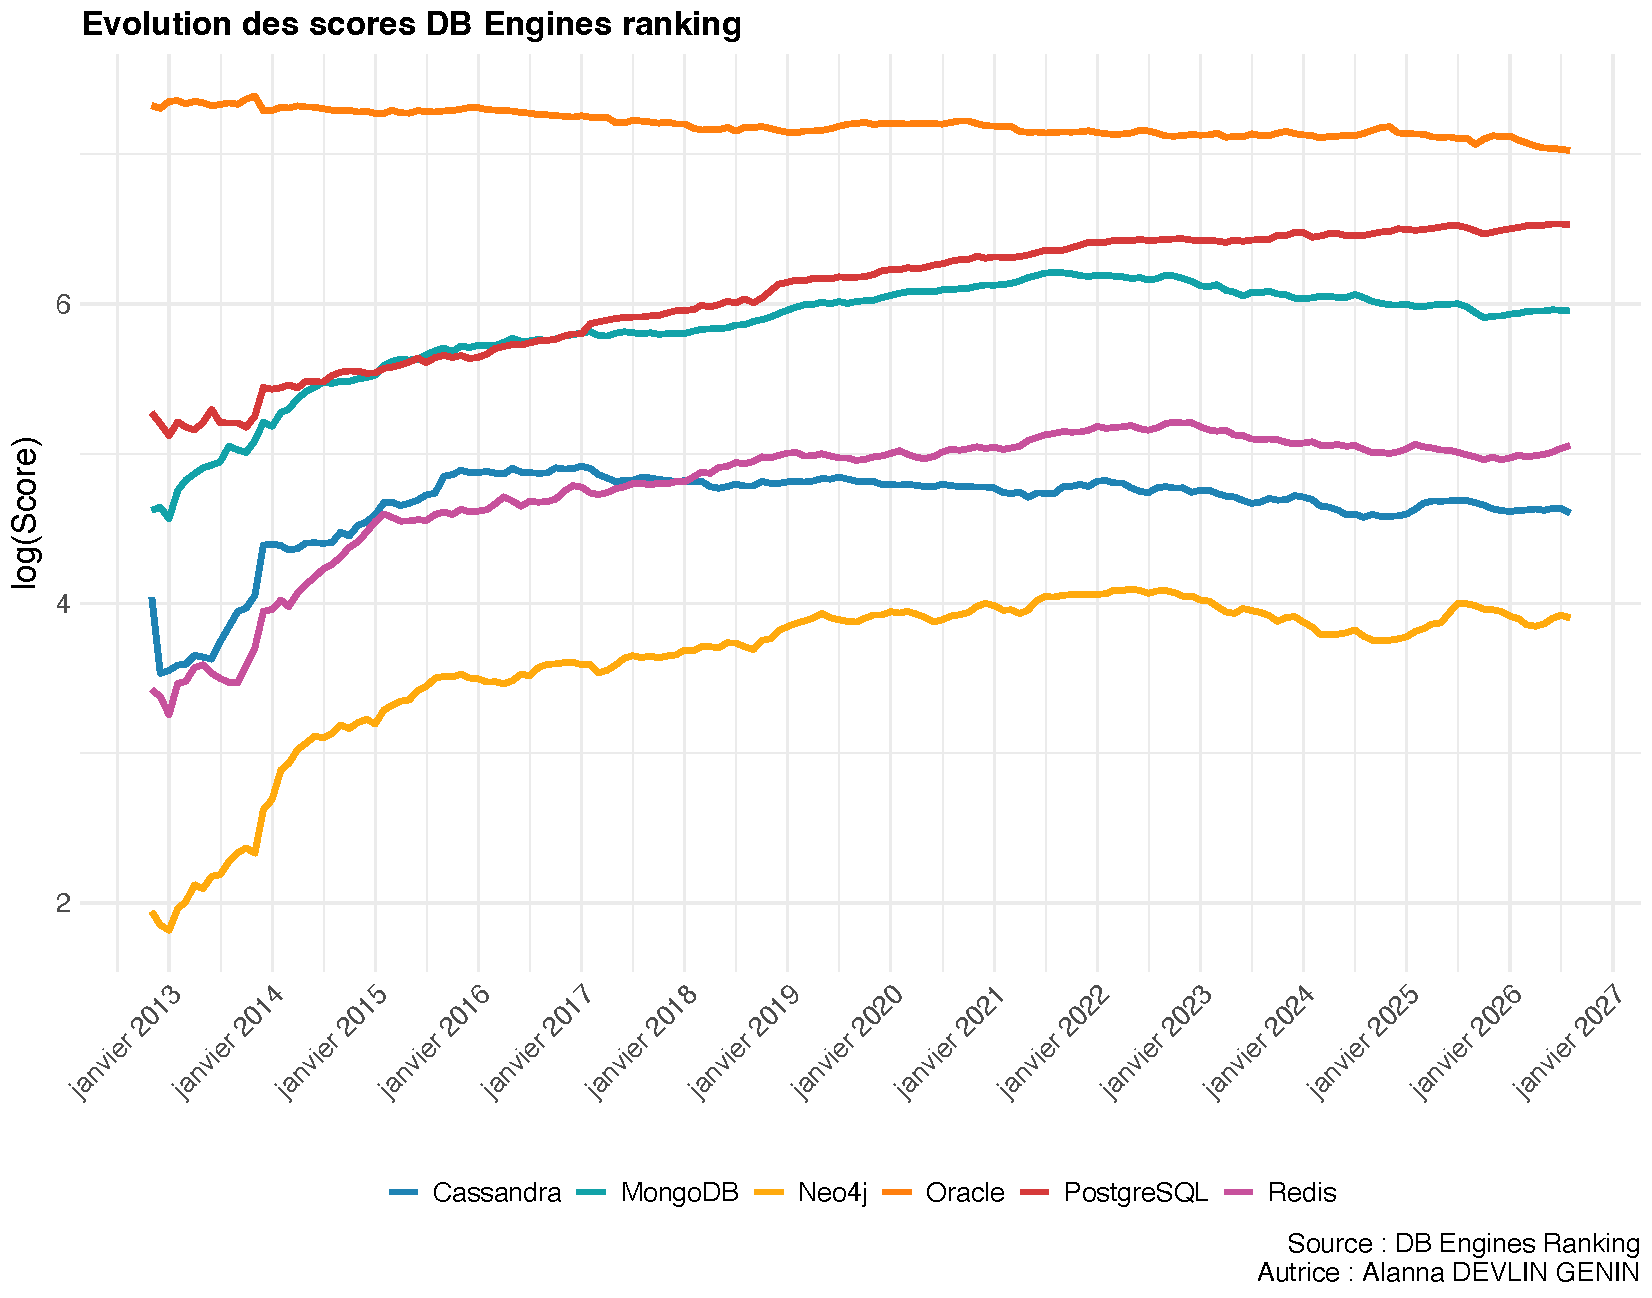
\includegraphics[width=0.85\textwidth]{img/nosql-db-engine.pdf}
    \end{figure}
\end{frame}

\begin{frame}{Popularité auprès des développeur$\cdot$euses}

    \begin{figure}[htb]
        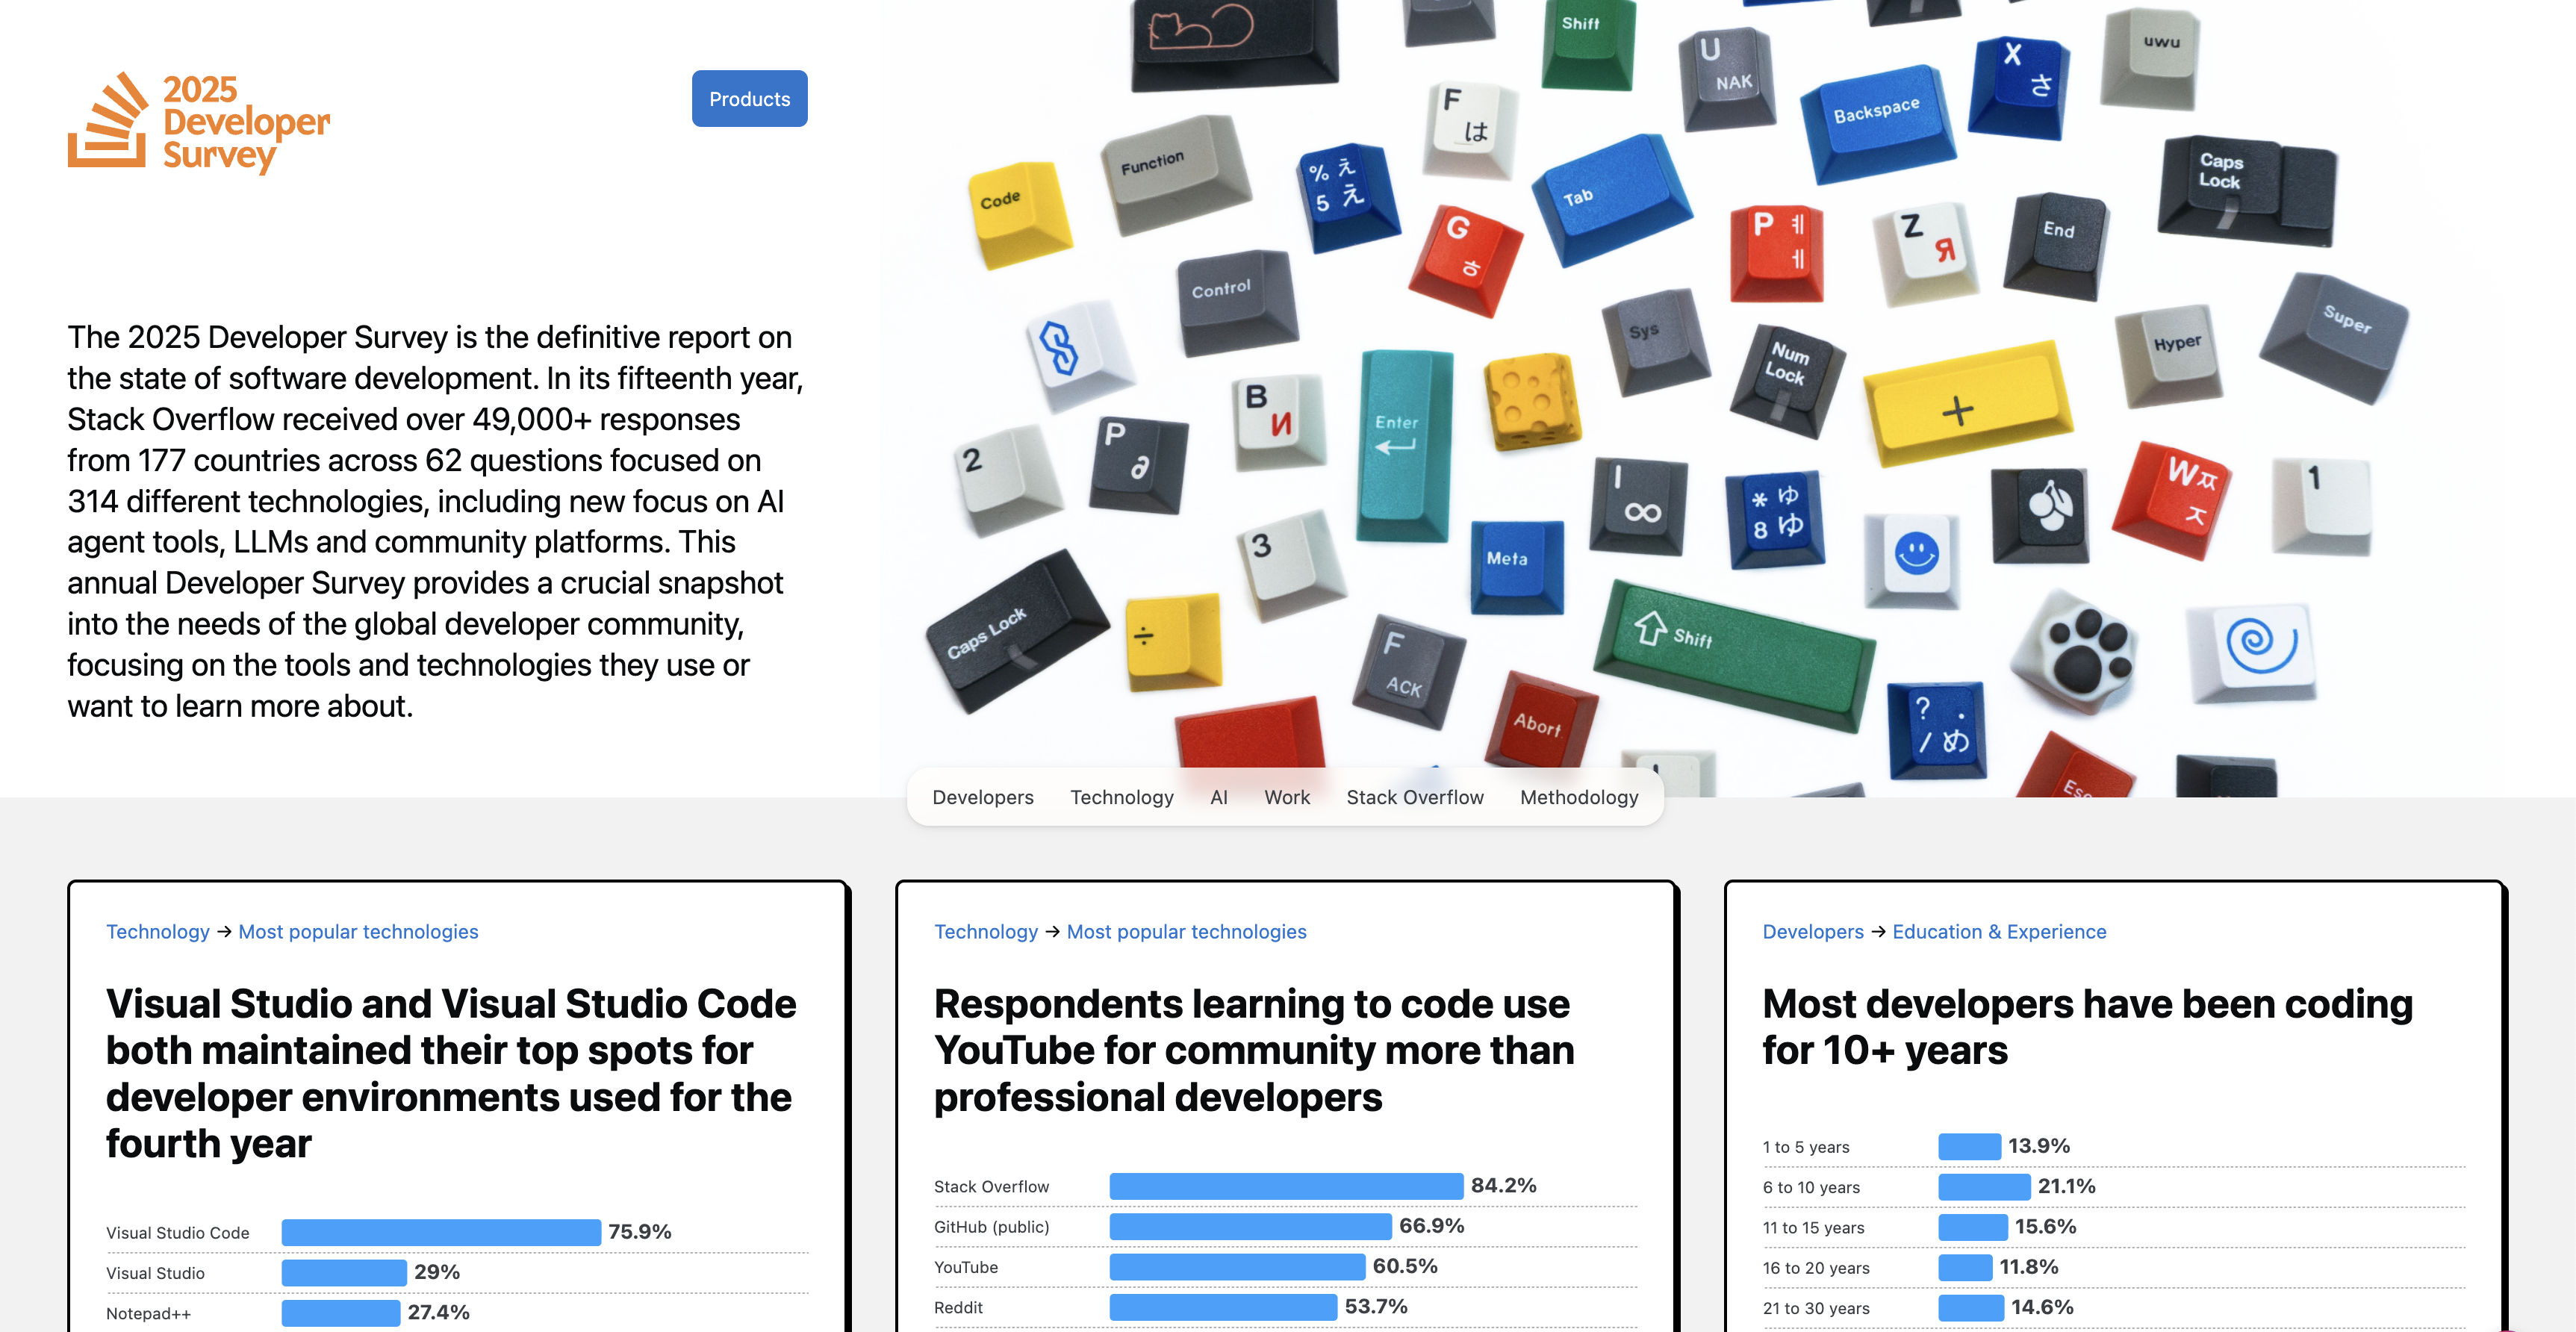
\includegraphics[width=\textwidth]{img/stack-overflow-survey-2025.png}
    \end{figure}

    \note{Enquête Stack Overflow (2025) : 60\% des développeur$\cdot$euses utilisent au moins une base NoSQL dans leurs projets, contre 45\% en 2020.}

\end{frame}

\begin{frame}{À quoi ça sert concrètement ?}

    \note{

    \begin{itemize}
        \item Flexibilité : Pas de schéma imposé → adaptation rapide aux changements de données.
        \item Performance : Lecture/écriture ultra-rapides, même avec des téraoctets de données.
        \item Scalabilité : Ajout facile de serveurs pour gérer la charge (ex : passer de 1 à 100 serveurs sans downtime).
        \item Coût : Moins cher à long terme pour les applications à forte croissance.
    \end{itemize}

    En résumé : NoSQL, c’est la réponse aux besoins modernes : données massives, variées, en temps réel, et applications qui montent en charge sans limite.
    }

\end{frame}

\begin{frame}{Cas d'utilisation de NoSQL}

    \begin{tikzpicture}
        \node[inner sep=0pt, label=below:Réseaux sociaux] (social) at (0,0)
            {
\includegraphics[width=.2\textwidth]{img/icon/social-media.png}};

        \node[inner sep=0pt, label=below:IoT, right=of social, xshift=1cm] (iot)
            {
\includegraphics[width=.2\textwidth]{img/icon/iot.png}};

        \node[inner sep=0pt, label=below:Personnalisation, right=of iot, xshift=1cm] (personnalisation)
            {
\includegraphics[width=.2\textwidth]{img/icon/customisation.png}};
    \end{tikzpicture}

     \note{
         \textbf{Réseaux sociaux} : Millions de likes/commentaires par seconde, données sociales non structurées (posts, images, vidéos).\\
         \textbf{IoT} : Des milliards de capteurs envoient des données en temps réel (température, localisation, etc.).\\
         \textbf{Personnalisation} : Analyse en temps réel des comportements utilisateurs pour recommander du contenu (Netflix, Amazon).\\
     }

\end{frame}

\begin{frame}{Cas concret : Netflix}
    % https://netflixtechblog.com/nosql-at-netflix-e937b660b4c

    \begin{figure}[htb]
        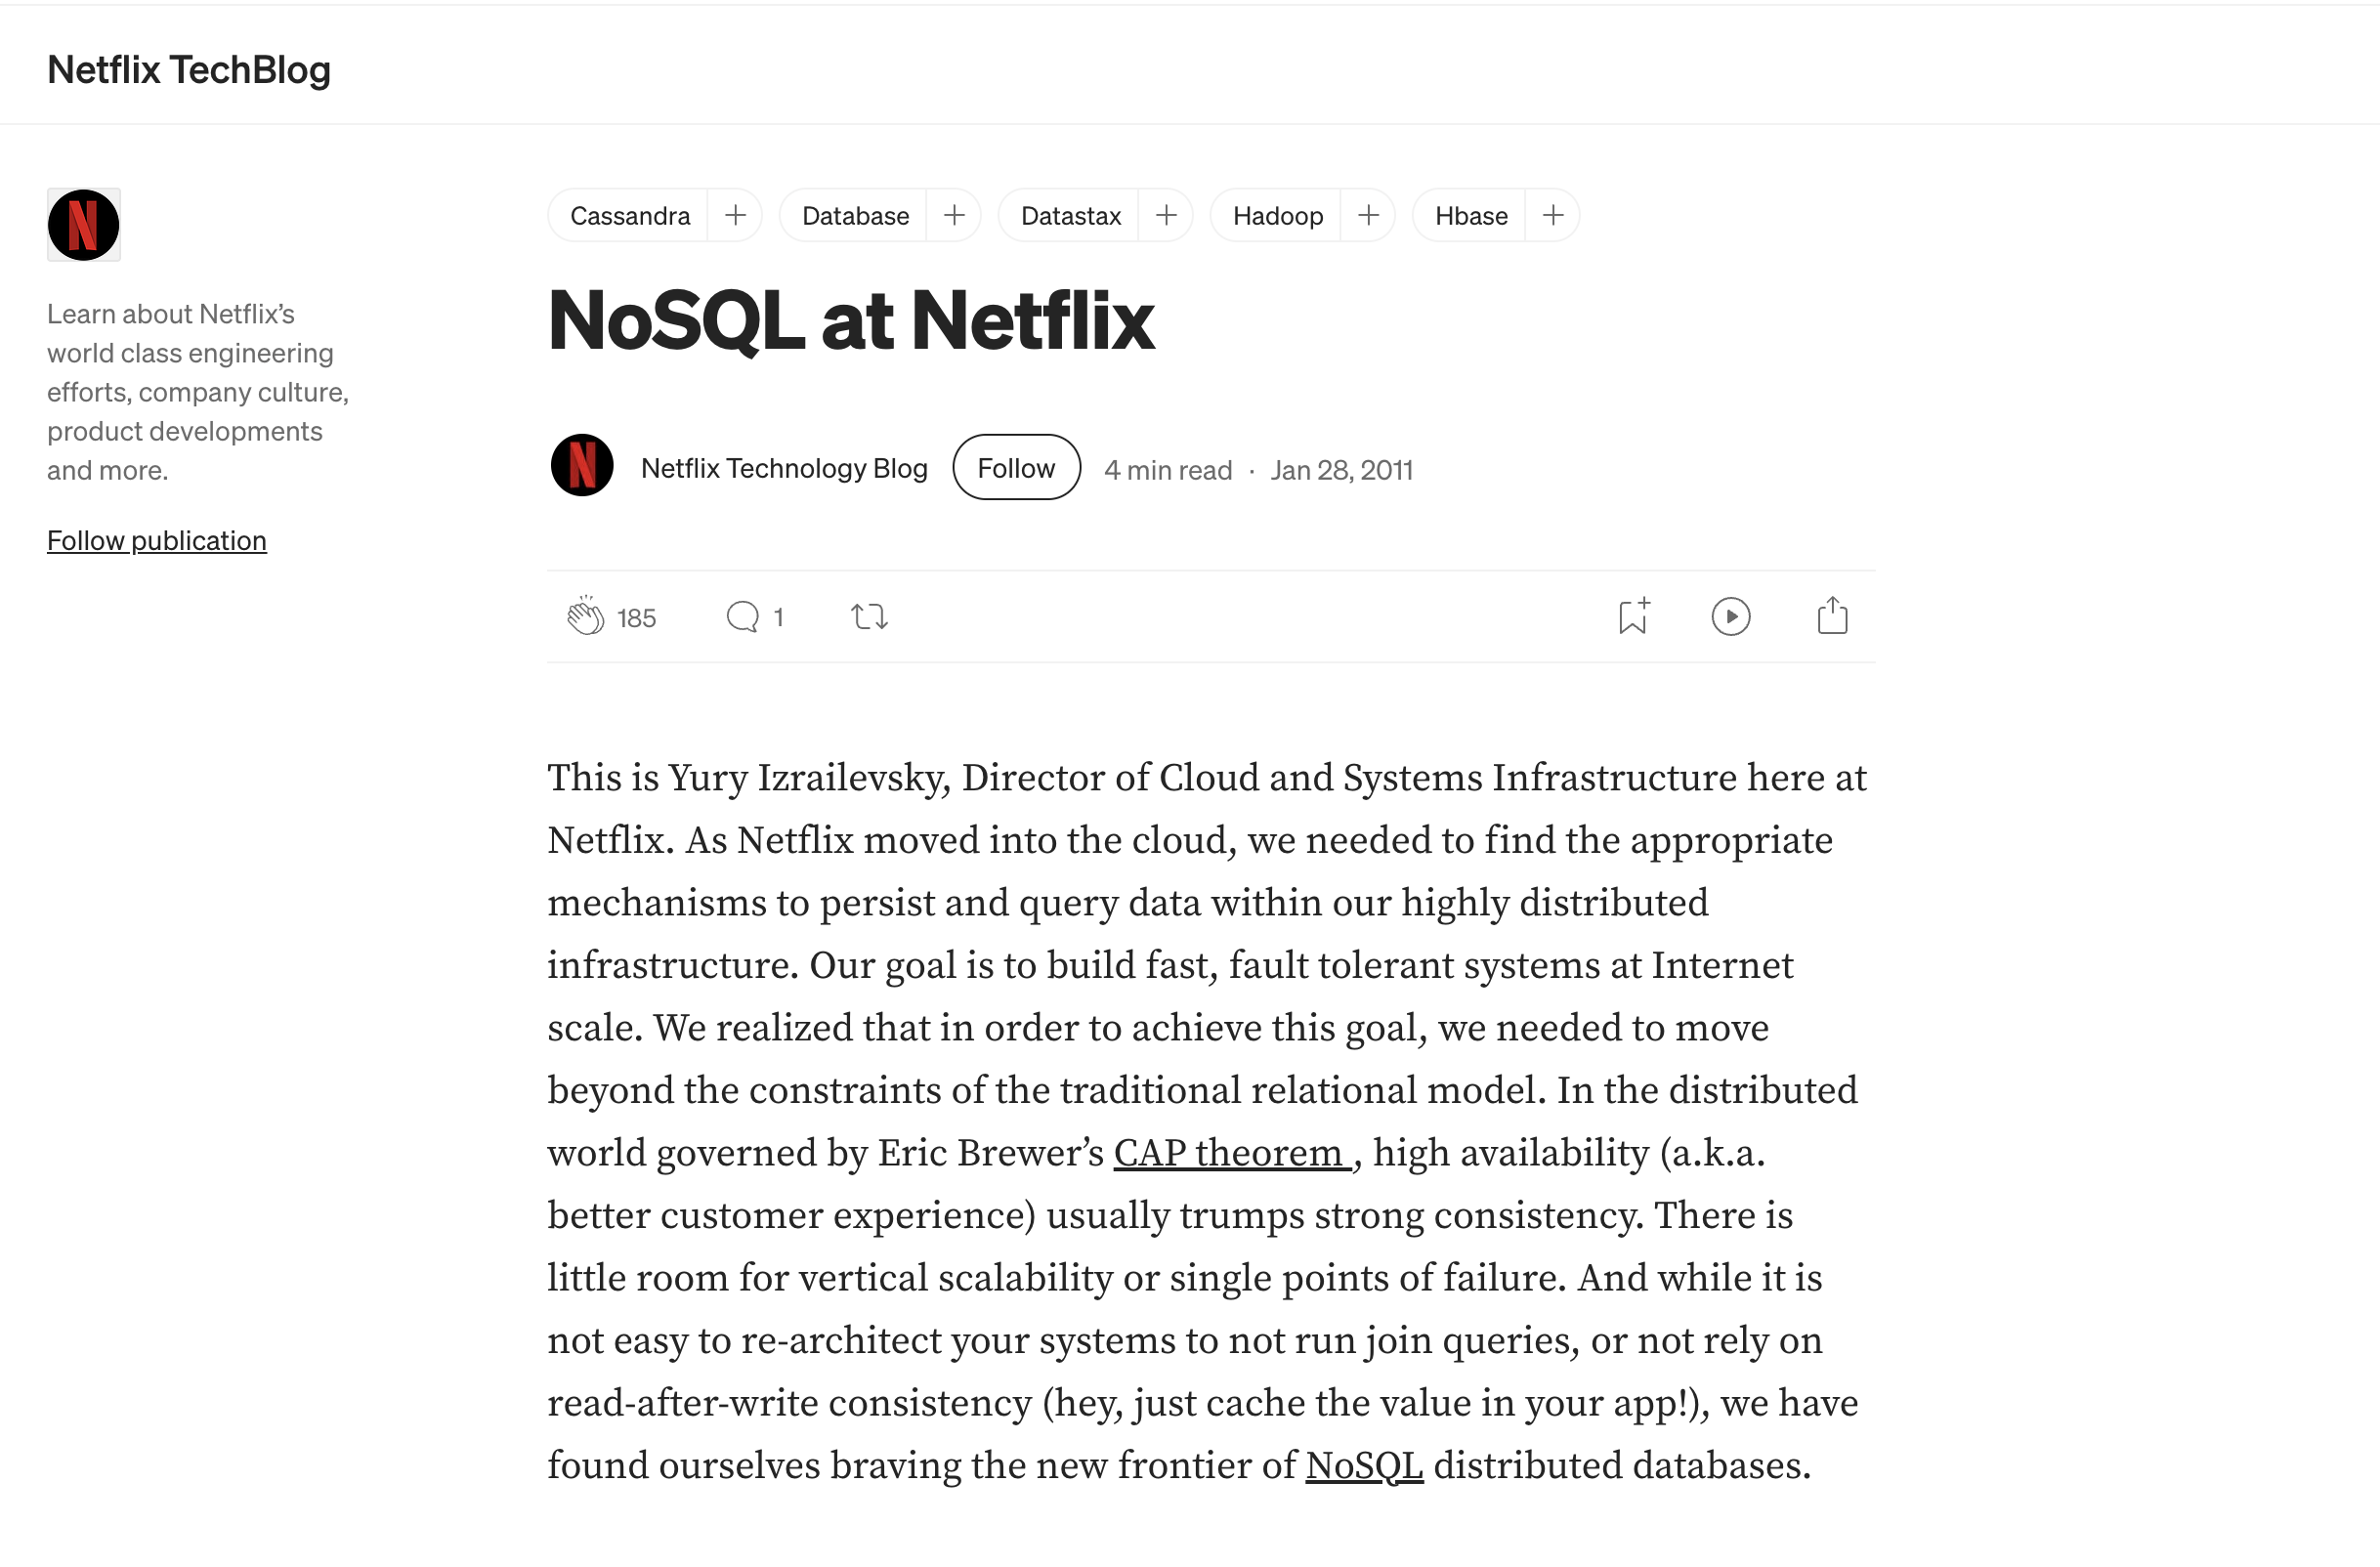
\includegraphics[width=\textwidth]{img/netflix-usecase.png}
    \end{figure}

    \note{
        Stockage des préférences utilisateurs, recommandations\\
        Cassandra, Amazon DynamoDB
    }

\end{frame}

\begin{frame}{Cas concret : Spotify}
    % https://engineering.atspotify.com/2015/1/personalization-at-spotify-using-cassandra

    \begin{figure}[htb]
        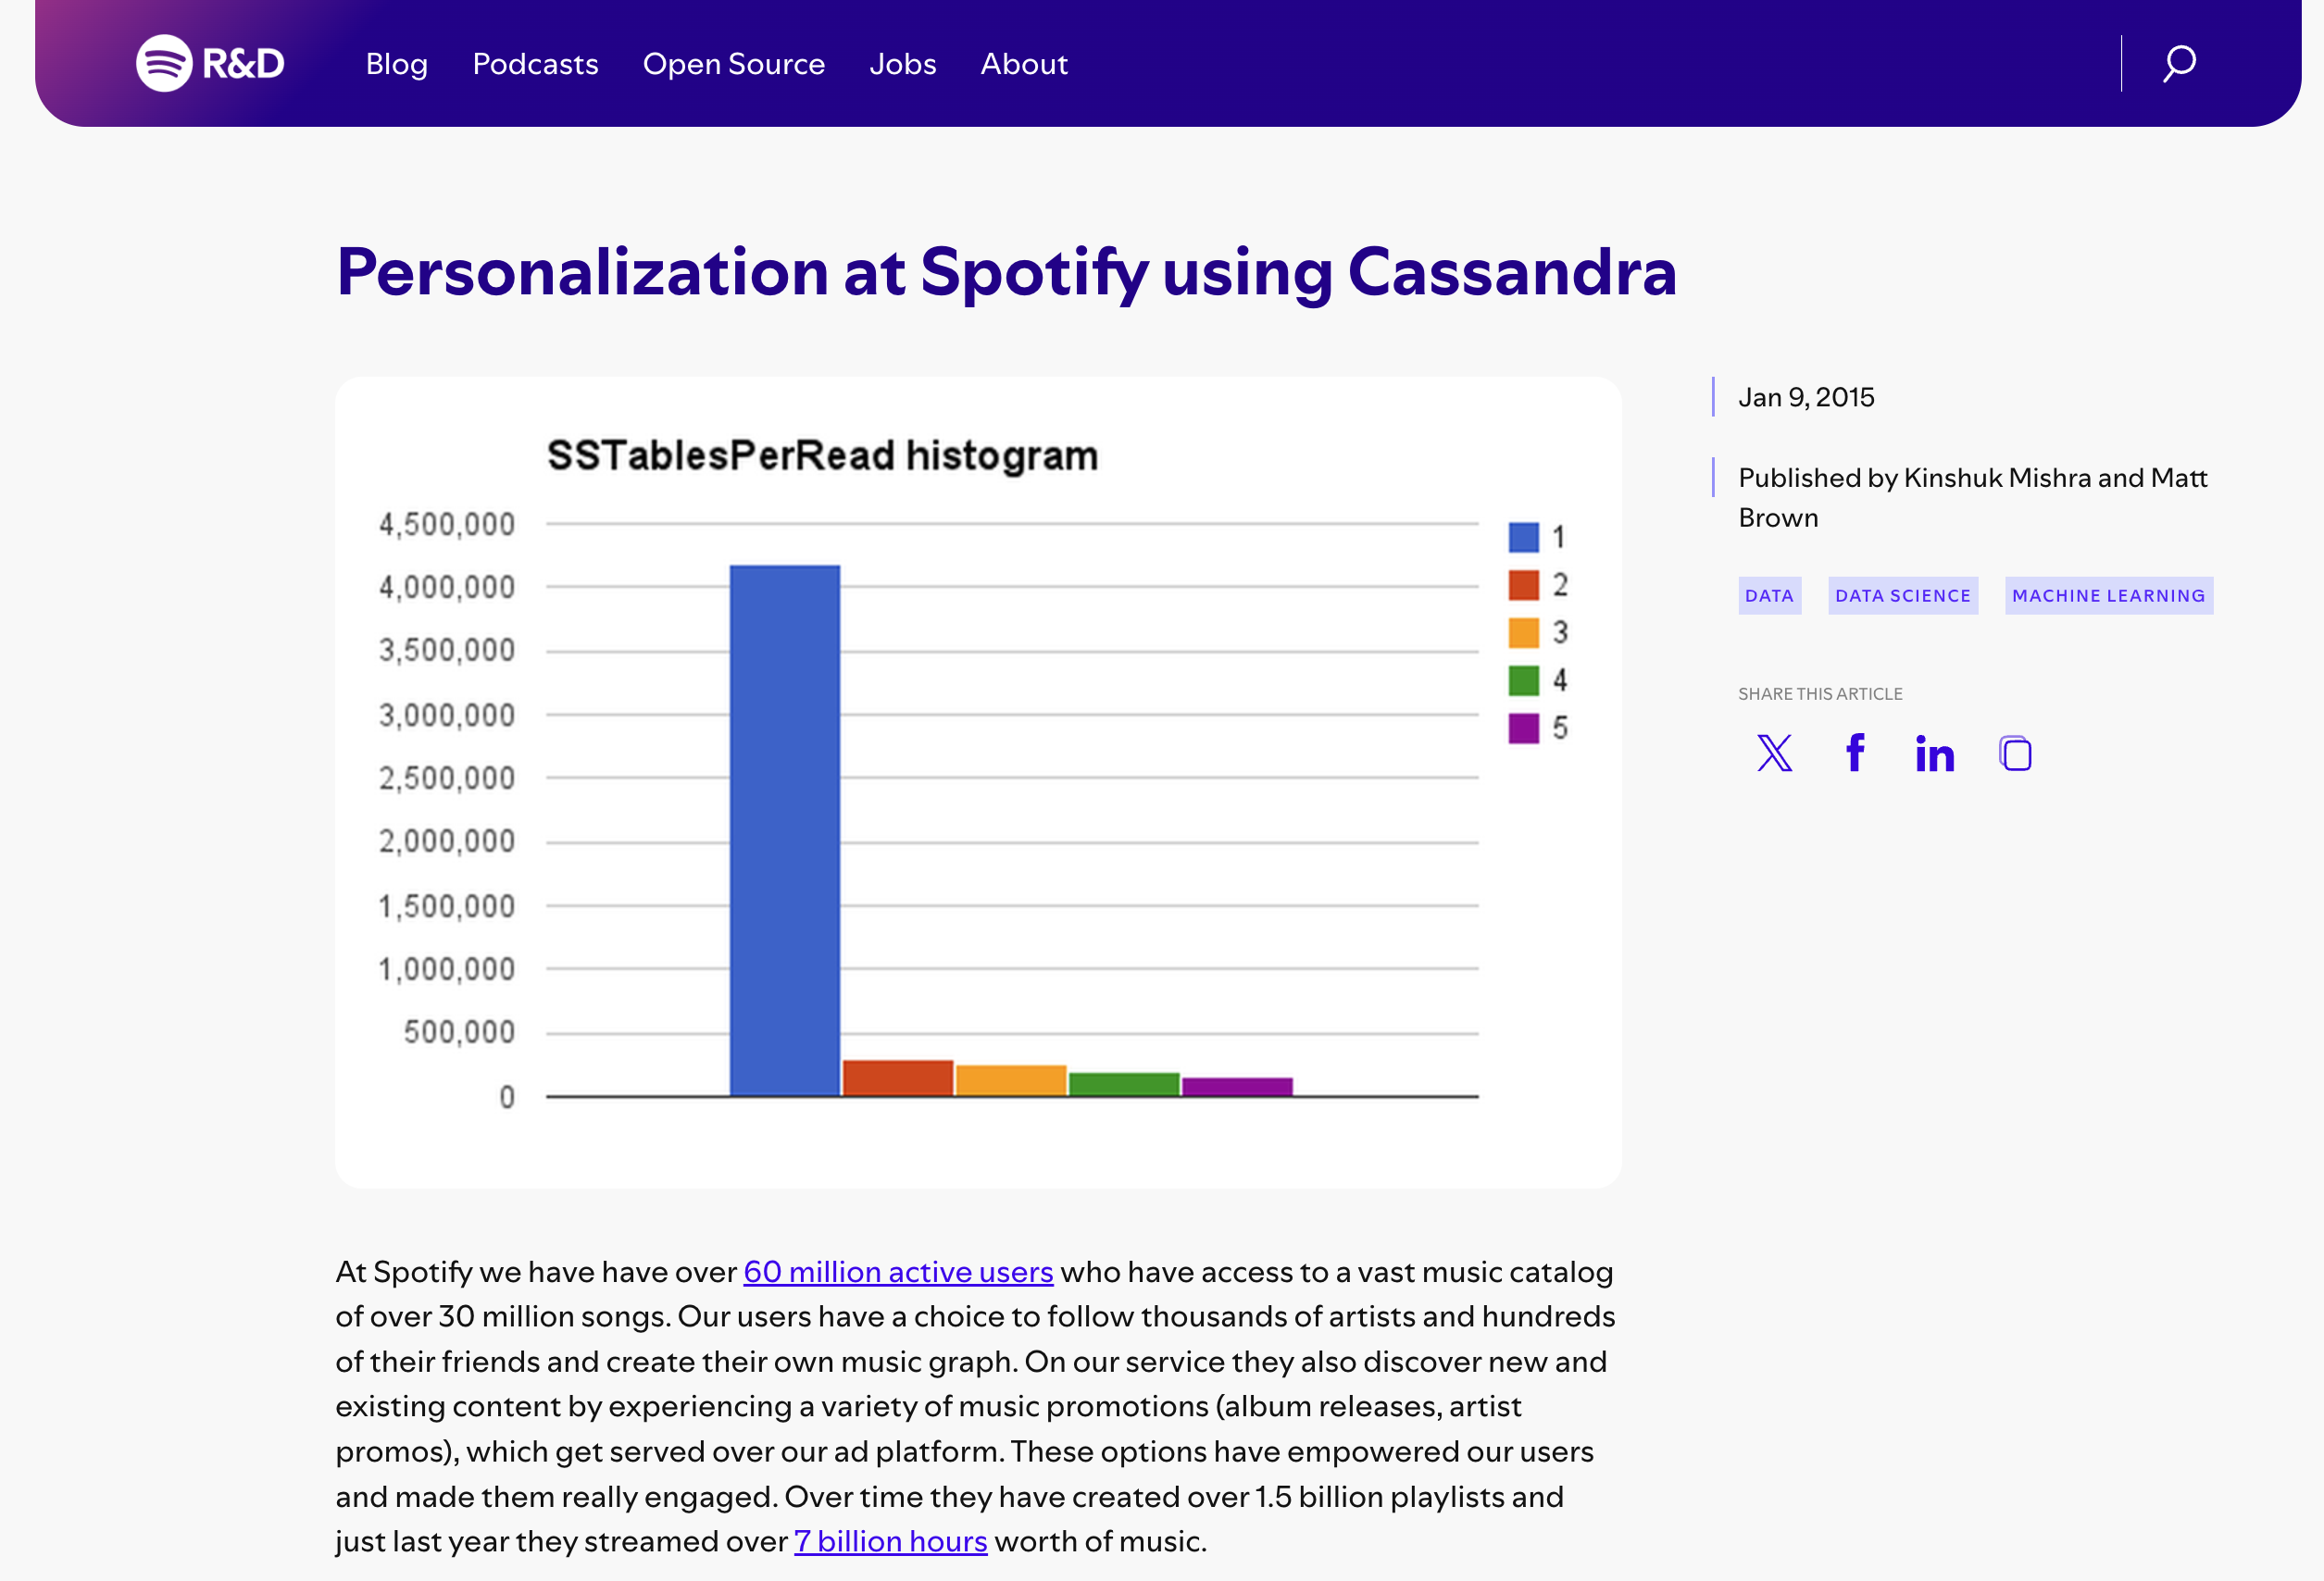
\includegraphics[width=\textwidth]{img/spotify-usecase.png}
    \end{figure}

    \note{
        Besoin : Personnaliser l'expérience utilisateur sur Spotify pour aider chaque client·e
        à découvrir du contenu pertinent selon son contexte et ses préférences, malgré
        l'abondance de choix et la diversité des comportements. \\
        Cassandra
    }

\end{frame}

\begin{frame}{Cas concret : L'Oréal}
    % https://www.mongodb.com/solutions/customer-case-studies/loreal

    \begin{figure}[htb]
        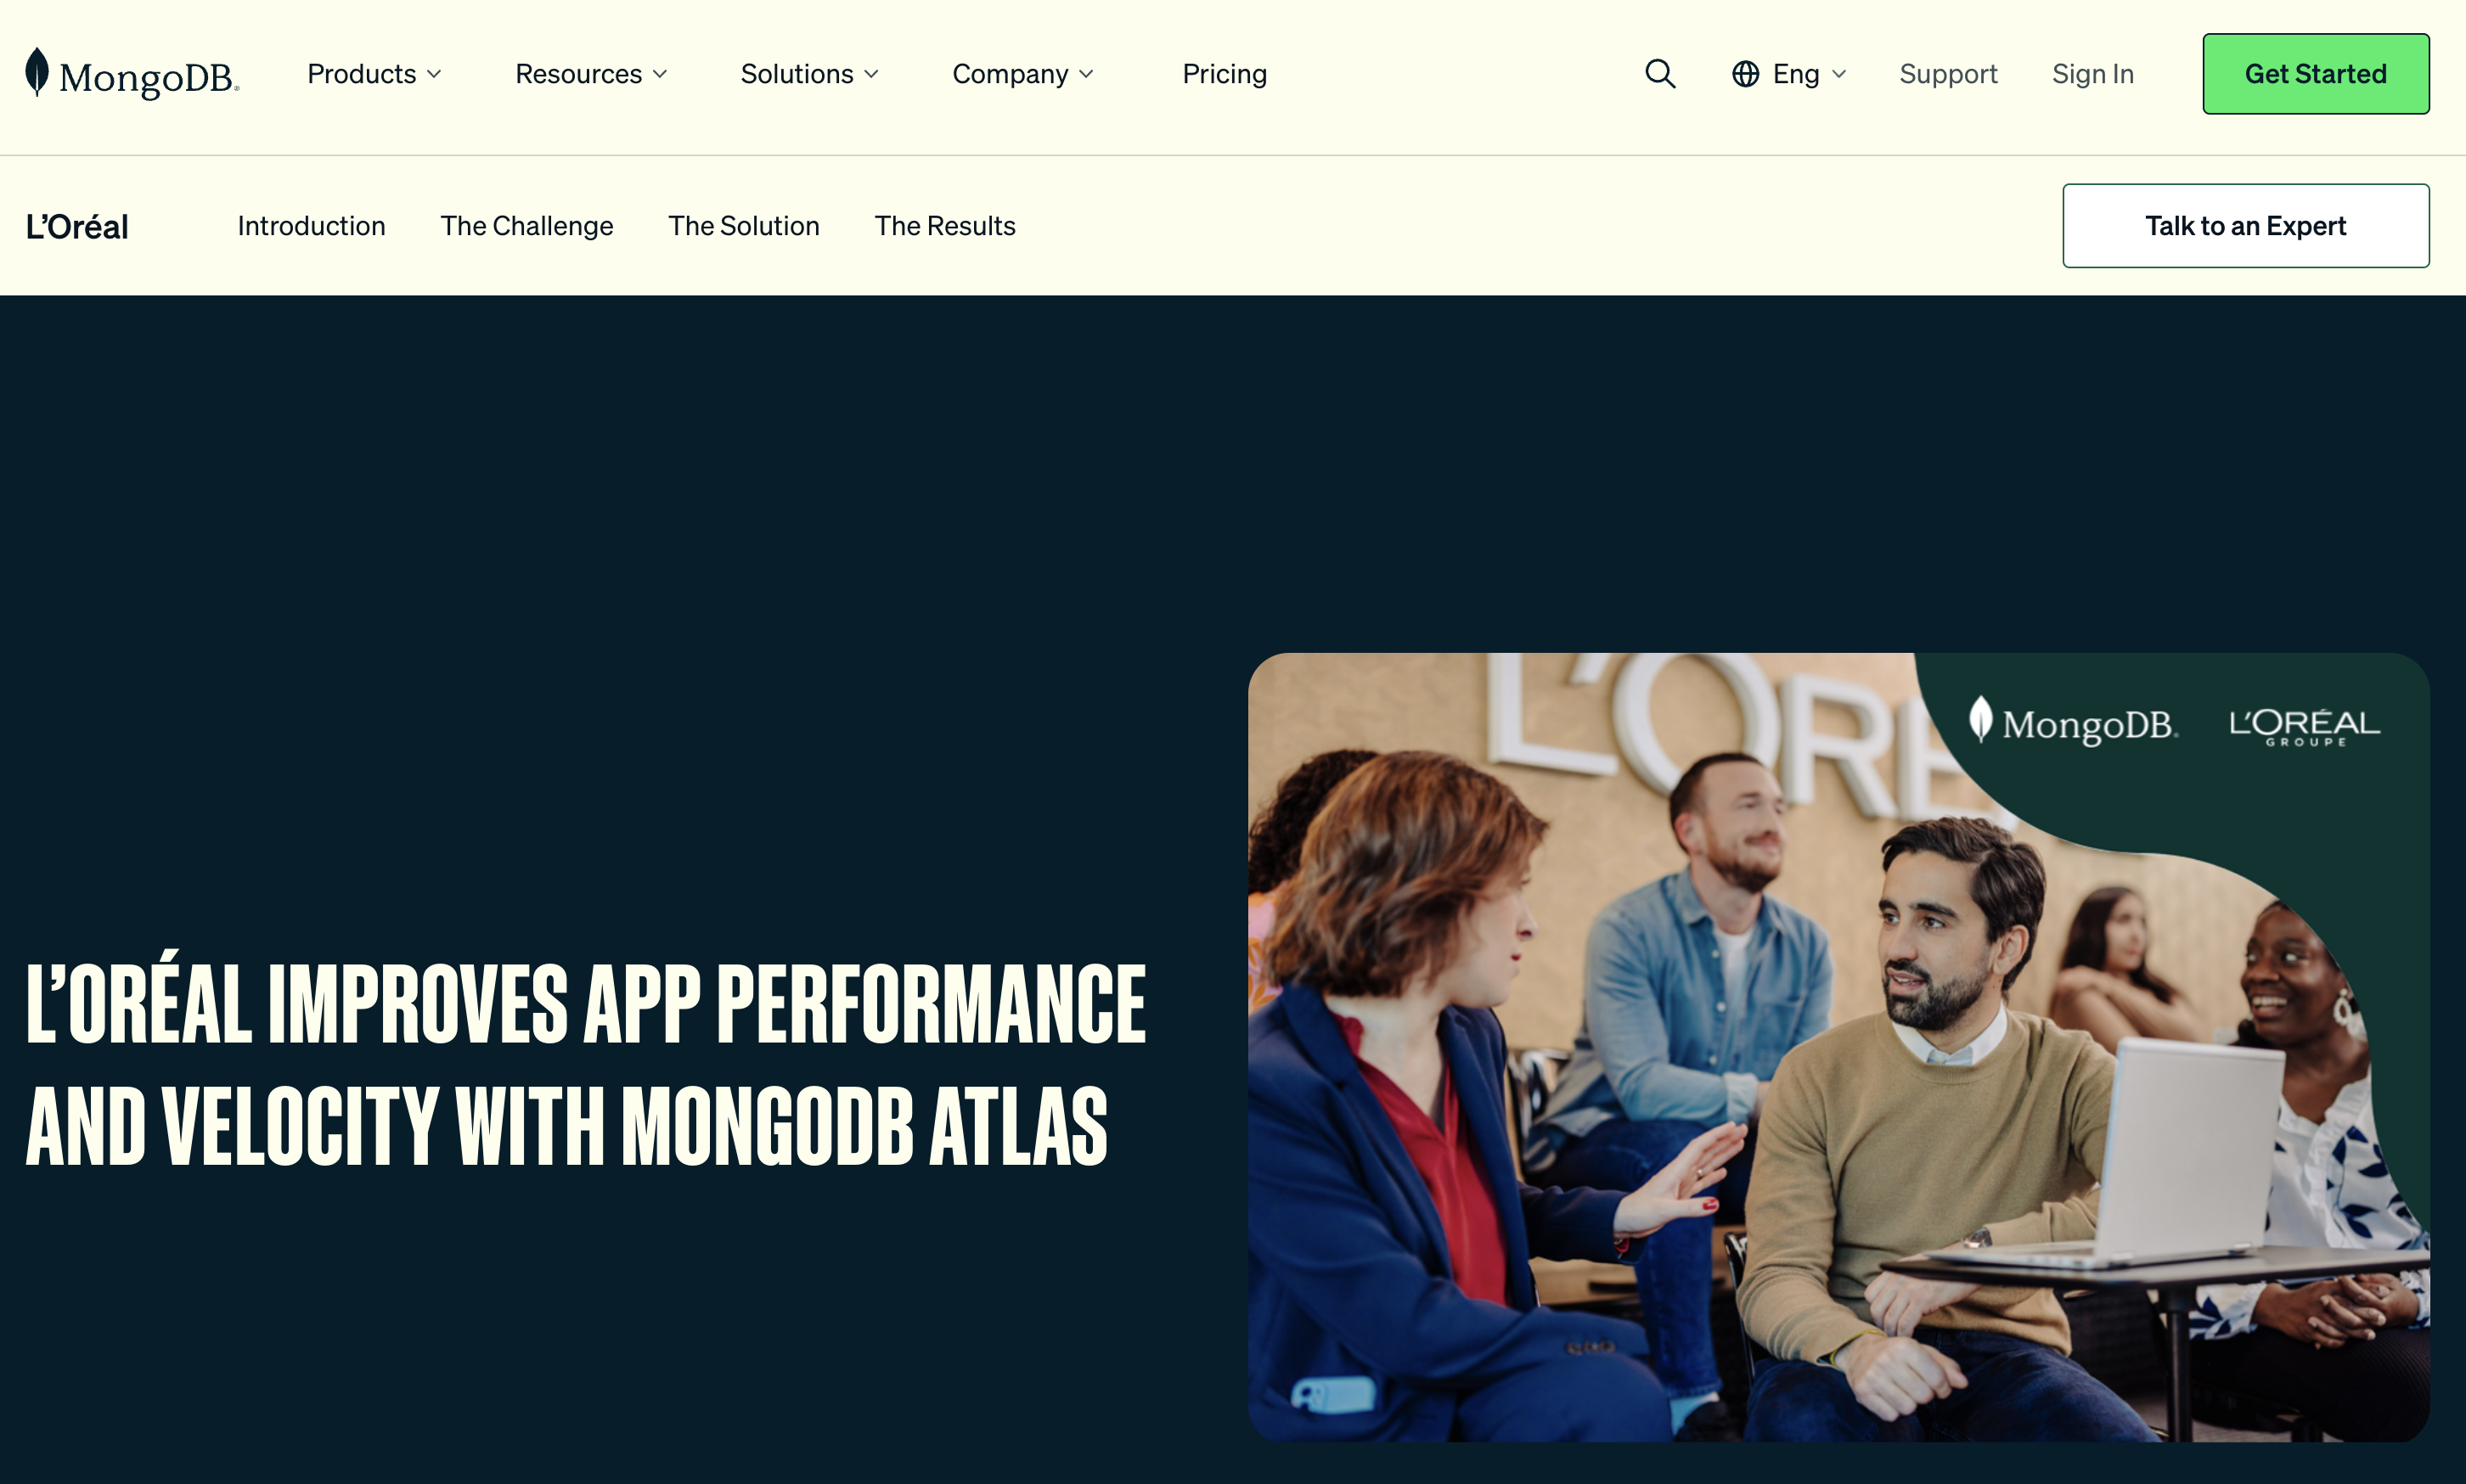
\includegraphics[width=\textwidth]{img/loreal-usecase.png}
    \end{figure}

    \note{
        Besoin : Calculs complexes en temps réel sur d’énormes volumes de données, sans aucun temps de latence \\

        L'une des solutions internes devait permettre de se connecter à plusieurs sources de données et de rechercher des corrélations afin de conseiller le personnel sur la manière de prendre des décisions stratégiques plus efficaces. Cela implique de stocker de grands volumes de données tout en effectuant des calculs et des analyses en temps réel.\\

        Résultat : Réduction de la latence de plusieurs secondes à 10 millisecondes \\

        MongoDB
    }

\end{frame}
